%%=============================================================================
%% Inleiding
%%=============================================================================

\chapter{Inleiding}
\label{ch:inleiding}

%%De inleiding moet de lezer alle nodige informatie verschaffen om het onderwerp te begrijpen zonder nog externe werken te moeten raadplegen \autocite{Pollefliet2011}. Dit is een doorlopende tekst die gebaseerd is op al wat je over het onderwerp gelezen hebt (literatuuronderzoek).

%%Je verwijst bij elke bewering die je doet, vakterm die je introduceert, enz. naar je bronnen. In \LaTeX{} kan dat met het commando \texttt{$\backslash${textcite\{\}}} of \texttt{$\backslash${autocite\{\}}}. Als argument van het commando geef je de ``sleutel'' van een ``record'' in een bibliografische databank in het Bib\TeX{}-formaat (een tekstbestand). Als je expliciet naar de auteur verwijst in de zin, gebruik je \texttt{$\backslash${}textcite\{\}}.
%%Soms wil je de auteur niet expliciet vernoemen, dan gebruik je \texttt{$\backslash${}autocite\{\}}. Hieronder een voorbeeld van elk.

%%\textcite{Knuth1998} schreef een van de standaardwerken over sorteer- en zoekalgoritmen. Experten zijn het erover eens dat cloud computing een interessante opportuniteit vormen, zowel voor gebruikers als voor dienstverleners op vlak van informatietechnologie~\autocite{Creeger2009}.

Voor 22 februari 2017 kon men dus enkel Docker installeren op Linux besturingssystemen. Dit dwong een onderneming die wou evolueren naar een DevOps manier van werken die geen kennis had van Linux om, ofwel iemand aan te schaffen die dit wel had of dat er een spoedcursus Linux moest gevolgd worden. Maar, met de komst van Windows 10 en Windows Server 2016, en de daarmee gepaard gaande groei van PowerShell en Hyper-V, is Docker nu ook toegankelijk voor organisaties die meer Windows gezind willen zijn. ~\autocite{DockerFAQ}

Want, het zou een vergissing zijn om Docker zomaar te negeren als je de DevOps richting uit wilt gaan. Het biedt immers verschillende gereedschappen aan voor zowel je developers als je sys admins. Bijvoorbeeld, Containers as a Service (CaaS) en role-based access control voor Operations, en een zelfbedienings-manier van werken voor Developers waarbij ze services kunnen opvragen wanneer zij ze nodig hebben. Momenteel wordt Docker dan ook gebruikt in 44 procent van de ondernemingen die van plan zijn om de DevOps richting in te slaan. ~\autocite{DockerDevOps}

\section{Stand van zaken}
\label{sec:stand-van-zaken}

%% TODO: deze sectie (die je kan opsplitsen in verschillende secties) bevat je
%% literatuurstudie. Vergeet niet telkens je bronnen te vermelden!
\subsection{DevOps}
\label{sec:devops-uitleg}
DevOps is een geclipte verbinding van de woorden 'Development' en 'Operations', je ontwikkeling en beheer. Voorheen werkte deze IT groepering strikt gescheiden, waardoor je ofwel bij de ene groep zat ofwel bij de andere. Dit zorgt ervoor dat, als men een applicatie wil maken, de developers het ontwikkelen en die dan richting de systeembeheerders werpen zodra de applicatie klaar is. Als de systeem beheerders hierna nog problemen hebben met de applicatie uitgerold te krijgen op hun servers, verloopt de communicatie altijd stroef door al het vinger wijzen dat er zal gebeuren. De applicatie werkte immers op de computers van de developers, de systeem beheerders moeten nu maar zien dat alles werkt op hun servers. Aangezien beide kanten dus niet veel weet hebben van elkaars werk, zorgt dit al snel voor wrevel.

\begin{center}
	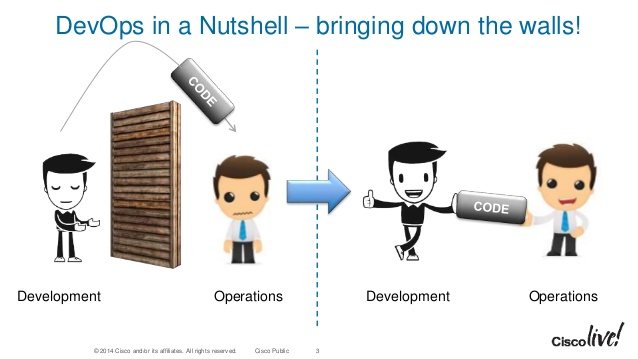
\includegraphics[scale=0.5]{img/devopsmuur.jpg}
\end{center}

Bij DevOps worden deze groepen gedwongen om samen te werken in één team. Zodat je samengevoegd een som krijgt die groter is dan het geheel. In praktijk vertaald dit zich naar een cultuur die gestimuleerd dient te worden, waarin het automatiseren van zoveel mogelijk zaken centraal staat met een focus op continue ontwikkeling en oplevering. Waarbij leren en het delen van informatie, en communicatie in het algemeen, zeer belangrijk is. Er worden ook verschillende manieren voorzien om informatie te verzamelen uit de applicatie, door methodes te implementeren die men gebruikt om zo een doorzichtiger systeem te hebben. Het is dus eerder een groep van concepten en ideeën dat gegroeid is tot een beweging dat snel tractie aan het winnen is.

Als éénduidige definitie voor DevOps kom je er het dichts bij met het acroniem 'CALMS'.
\begin{itemize}[noitemsep]
	\item Culture (Cultuur)
	\item Automatisation (Automatisatie)
	\item Learning (Leren, voorheen Lean)
	\item Measure (Meten)
	\item Sharing (Delen)
\end{itemize}

 ~\autocite{WhatIsDevOps}

\begin{center}
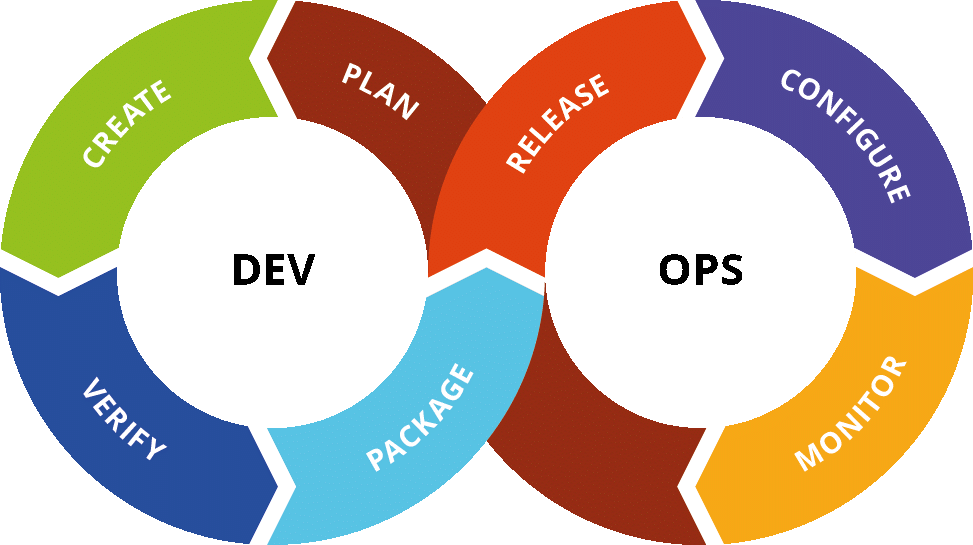
\includegraphics[scale=0.5]{img/devops.png}
\end{center}

\subsection{Docker}
\label{sec:docker-uitleg}
Docker is een gereedschap om het uitrollen van applicaties sneller en makkelijker te maken doordat het de applicatie, en alle benodigdheden, ervoor in één geautomatiseerd pakketje verpakt. Dat zal werken los van het host besturingssysteem. Dit pakket in zijn geheel wordt een container genoemd. ~\autocite{OpenSourceDocker}

Containers lijken op het eerste zicht hard op virtuele machines. Maar, belangrijk om te onthouden is dat de onderliggende architectuur sterk verschilt tussen de 2. De beste manier om ernaar te kijken is zoals naar appartementen en huizen. Een huis staat volledig op zich, en voorziet zelf in al zijn behoefte qua infrastructuur. Net zoals een huis zal de virtuele machine volledig onafhankelijk opgebouwd worden, los van je eigen host. Containers zijn zoals appartementen in dat ze de bestaande infrastructuur delen. Alle middelen van de host waar de Docker Host op geïnstalleerd wordt zullen worden gedeeld onder de verschillende containers. Waarbij, net zoals een appartement, elk aangeboden container voldoet aan de noden van zijn bewoner. ~\autocite{ContainerVsVM}

Een container zal hierdoor dus een lichtere en onafhankelijke uitvoerbaar software pakket kunnen opbouwen. Met de extra bonus dat het consistentie kan garanderen doordat er telkens gebruik zal gemaakt worden van dezelfde achterliggende images. ~\autocite{DockerContainer}

Doordat elk deel van een applicatie dus in zo'n appartementje zit, is het maken van continue ontwikkeling en oplevering voor de applicatie heel makkelijk te doen. Je moet immers alleen die specifieke container updaten/graden. Hierdoor is het de perfecte technologie om te dienen als productie- en testomgeving. Verder versoepelt het ook de communicatie in het DevOps-team doordat iedereen continue in dezelfde omgeving aan het werken is. Er zijn immers geen grote veranderingen nodig tijdens verschillende stappen van de leveringsketen. Verder maakt het ook nog het leven van iedereen makkelijker doordat je instaat bent op verschillende frameworks te draaien op één platform. Omdat de container vrij agnostisch zijn op vlak van programmeertaal of platform. Containers kunnen ook makkelijk van host besturingssysteem verplaatst worden.  ~\autocite{DevOpsContainers}

\begin{center}
	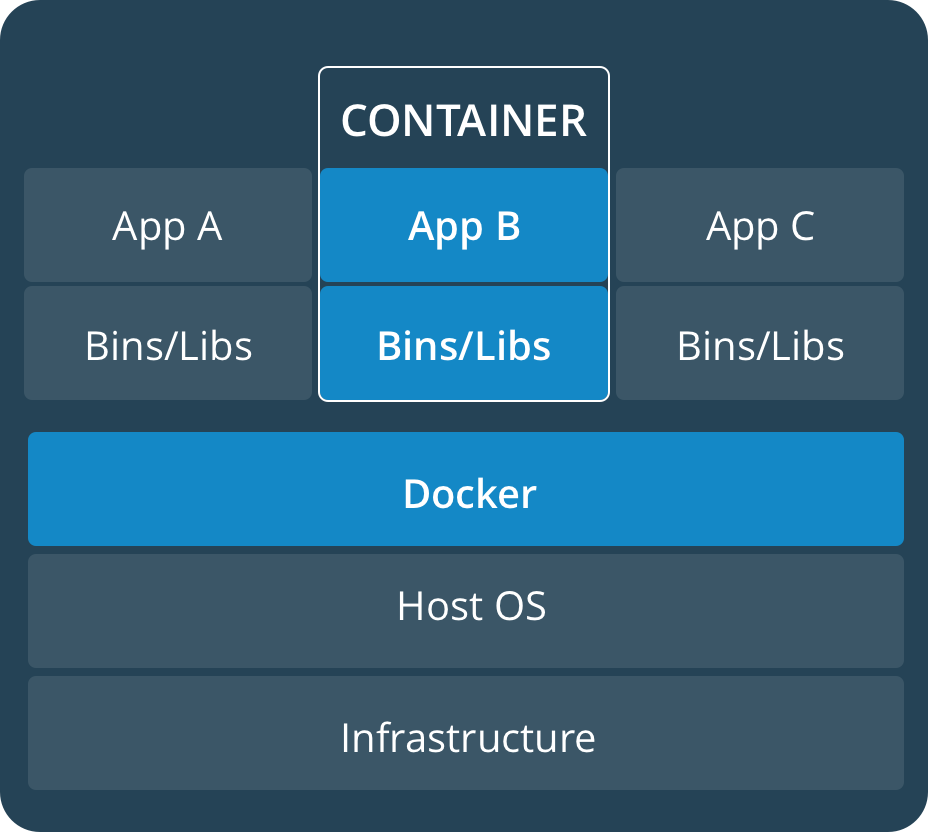
\includegraphics[scale=0.2]{img/containers.png}
	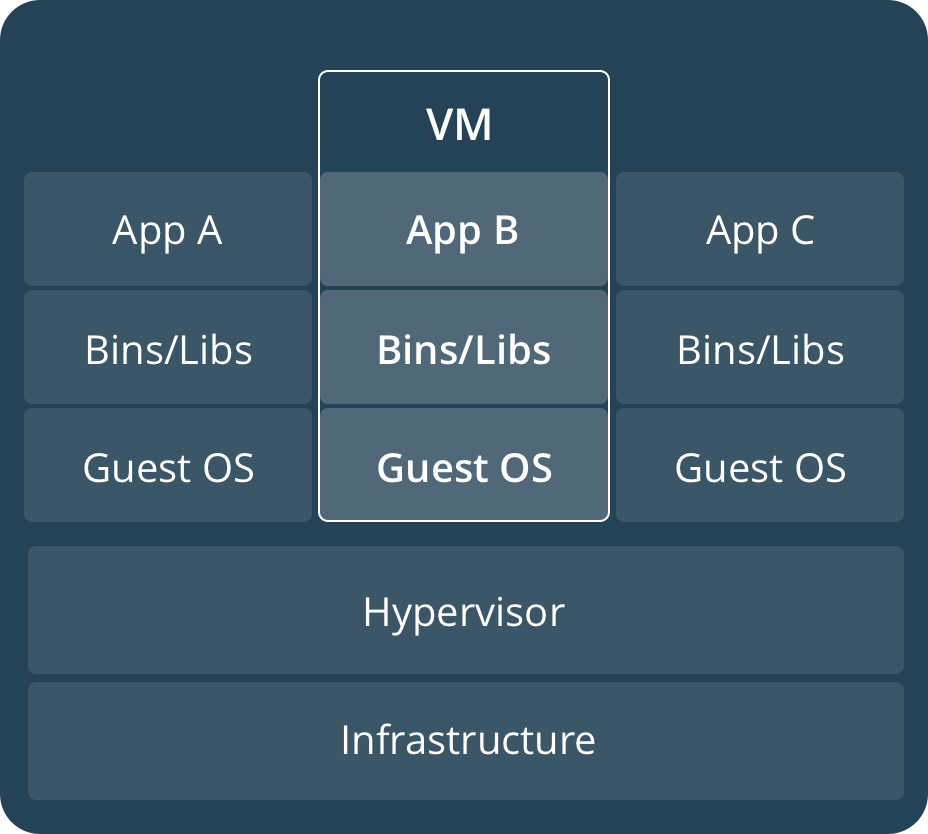
\includegraphics[scale=0.2]{img/vms.png}
\end{center}

%% Werking Docker

Het door al deze redenen dat Docker jaar na jaar blijft groeien. Tijdens de meest recentste DockerCon heeft de CEO van Docker enkele knallende cijfers kunnen tonen, zoals bijvoorbeeld:
\begin{itemize}[noitemsep]
	\item Meer dan 14 miljoen Docker hosts
	\item More dan 900.000 applicaties die draaien op Docker
	\item Een verhoging van 40 procent in het toepassen ervan in 1 jaar
\end{itemize}
~\autocite{DockerNumbers}

Docker heeft deze groei ook verdient. Door constant in contact te blijven met zijn gebruikers. In het verleden hadden ze immers de klacht gekregen dat ze ofwel te traag of te snel updates toevoegden aan het systeem. Om dit te remediëren hebben ze naast Docker Community Edition, waarmee alles is begonnen, nu ook Docker Enterprise Edition in het leven geroepen. Met daarbovenop een verschuiving naar een tijdgebaseerde updatesysteem. Waarbij je kunt kiezen tussen elke maand een update, maar zonder garantie op stabiliteit (Edge). Of, elke 4 maand een update, voor gebruikers die stabiliteit prefereren zowel op vlak van onderhoud als beheer (Stable). Daarbovenop heeft de Enterprise Edition ook een uitgebreidere ondersteuning met verschillende gradaties. ~\autocite{EEvCE}

\subsubsection{Docker CE}
Zoals eerder aangehaald is Docker CE het origineel platform waarmee ze zijn begonnen. Het is ideaal voor kleine teams of onafhankelijke developers die willen experimenteren met container technologie. Beschikbaar voor zowel Linux, Windows als Mac is het perfect als kleine en snelle installatie om direct aan de slag te gaan. Daarbovenop biedt het ook ondersteuning voor het uitrollen naar Cloud omgevingen, zoals Amazone Web Services of Azure. ~\autocite{DockerCE}

\subsubsection{Docker EE}
Docker Enterprise Edition is volledige pakket voor zij die op een professionele manier met een Containers-as-a-Serivce platform willen werken. Docker EE is dus een geïntegreerd en getest platform voor Linux of Windows Enterprise en Cloud providers, met door Docker gecertificeerde componenten en ondersteuning. In het bijzonder, is voor datacenters een handig dashboard waar ze hun multi-architecturaal orkestratie software supply chain kunnen volgen op een veilig manier. Vooral aan dat laatste heeft Docker extra veel aandacht besteedt met kenmerken zoals trusted delivery. ~\autocite{DockerEE}

\begin{center}
	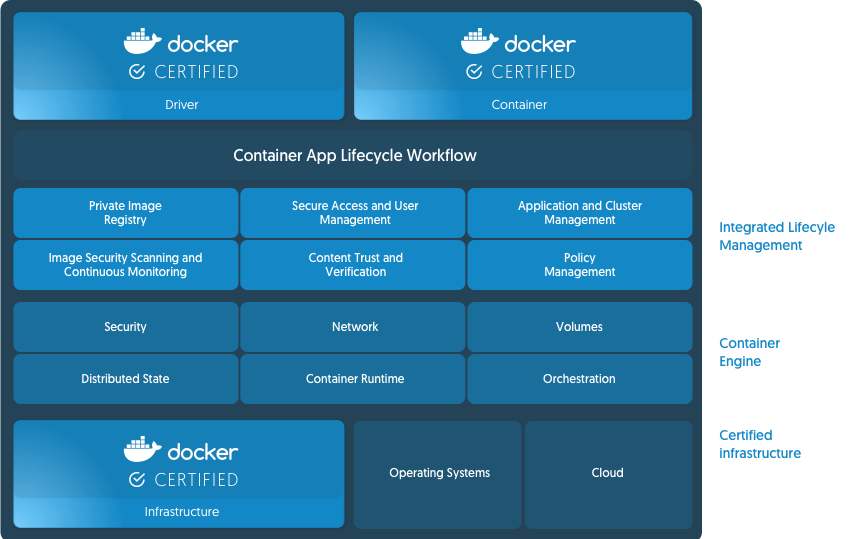
\includegraphics[scale=0.2]{img/dockerce.png}
\end{center}


%% Lagen software testing uitleggen
%% Beter verwoorden
%% Meer

\subsection{Software testing}
\label{sec:testing-uitleg}
In het hart van software testing ligt een focus op kwaliteit in alle delen van de organisatie. Dit is belangrijk om te weten omdat het ontwikkelingsteam verantwoordelijk is voor de kwaliteit. QA teams kunnen misschien op tijd aan de alarmbel trekken op vlak van risico's, maar men kan niet de verantwoordelijkheid van kwaliteit wegnemen van het ontwikkelingsproces. Daarom dat software testing eist dat iedereen, inclusief de gebruiker betrokken is bij het ontwikkelingsproces. ~\autocite{SoftwareTesting}

\begin{center}
	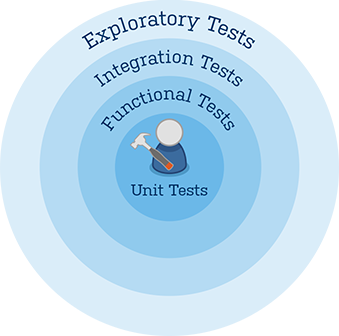
\includegraphics[scale=0.5]{img/testing.png}
\end{center}

~\textcite{CemKaner2006} zegt over software testing ook dat het een empirische en technische manier is om software of services te testen. Doordat er op een objectieve manier wordt gekeken naar de kwaliteit van een software of service. Het is vooral daarom dat er voor deze methode gekozen is geweest en het sluit ook heel goed aan bij de principes van het DevOps manifesto.
Specifiek zal er gebruik gemaakt worden van performantie-, integratie- en veiligheidstesten.
Performantietesten zijn een type van testen waarbij men gaat kijken hoe het systeem presteert wanneer het een bepaalde werkdruk moet verwerken, met een focus op snelheid, schaalbaarheid en stabiliteit. ~\autocite{PerformanceTesting}
Bij integratietesten ligt de focus op de datacommunicatie tussen de verschillende modules. In dit geval tussen Docker, het besturingssysteem van de host en de uitgerolde applicatie. ~\autocite{IntegrationTesting}
Bij veiligheidstesten zal er gekeken worden naar al de verschillende veiligheidsmaatregelen, in hoever ze instaat zijn om de zwaktes van het systeem te beschermen. ~\autocite{SecurityTesting}

\begin{center}
	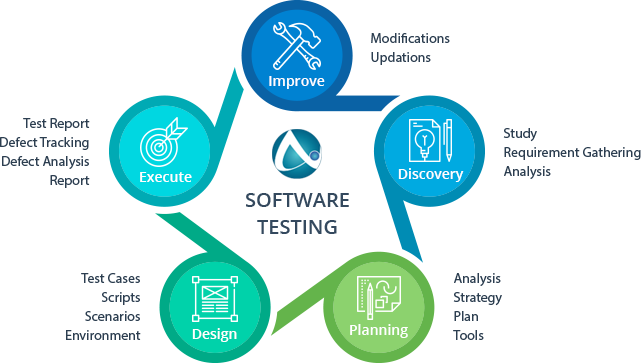
\includegraphics[scale=0.5]{img/testingprocess.png}
\end{center}

\section{Probleemstelling en Onderzoeksvragen}
\label{sec:onderzoeksvragen}

%% TODO:
%% Uit je probleemstelling moet duidelijk zijn dat je onderzoek een meerwaarde
%% heeft voor een concrete doelgroep (bv. een bedrijf).
%%
%% Wees zo concreet mogelijk bij het formuleren van je
%% onderzoeksvra(a)g(en). Een onderzoeksvraag is trouwens iets waar nog
%% niemand op dit moment een antwoord heeft (voor zover je kan nagaan).

De probleemstelling die zich voordoet is dat Docker op zich nog een, relatief, jonge technologie is, met daarbovenop een eigen syntaxis en verandering van werken en denken vereist om het op een goede manier te beheersen. Stap bij stap zijn Linux administrators er ondertussen vertrouwd mee aan het geraken. Maar, voor Windows administrators is dit een gloednieuwe technologie.


De onderzoeksvragen die uit deze probleemstelling dan voortvloeien luiden als volgt:
\begin{itemize}[noitemsep]
	\item Hoe vlot kan men een Docker opstelling maken op een Windows tegenover op een Linux besturingssysteem?
	\item Hoe is het gesteld met de documentatie voor Docker for Windows tegenover de bestaande documentatie voor Linux?
	\item Een groot voordeel van Docker is de snelheidswinst. Hoe groot is deze op Windows?
	\item Hoe goed is technologie geïntegreerd met Hyper-V en het Windows besturingssysteem in het algemeen?
	\item Hoe is het gesteld met de veiligheid? Hoe pak je deze aan vanuit een Windows administrator perspectief?
\end{itemize}


Voor al deze vragen kon er tot op heden nog geen afdoend antwoord voor gevonden worden. Er hebben wel al verschillende gebruikers Docker for Windows uitgetest en vergeleken met Linux. Maar, nooit op een concrete en methodische manier. Vaak benaderden ze deze technologie ook vanuit een bestaande mening, en niet met een neutraal perspectief.


Dit onderzoek zal vooral een grote meerwaarde zijn voor DevOps teams die op zoek zijn naar een Windows oplossingen voor hun problemen in verband automatisatie en continue oplevering.

\section{Opzet van deze bachelorproef}
\label{sec:opzet-bachelorproef}

%% TODO: Het is gebruikelijk aan het einde van de inleiding een overzicht te
%% geven van de opbouw van de rest van de tekst. Deze sectie bevat al een aanzet
%% die je kan aanvullen/aanpassen in functie van je eigen tekst.

De rest van deze bachelorproef is als volgt opgebouwd:

In Hoofdstuk~\ref{ch:methodologie} wordt de methodologie toegelicht en worden de gebruikte onderzoekstechnieken besproken om een antwoord te kunnen formuleren op de onderzoeksvragen.

%% TODO: Vul hier aan voor je eigen hoofstukken, één of twee zinnen per hoofdstuk

In Hoofdstuk~\ref{ch:opstelling} worden beide opstellingen bekeken en besproken. Namelijk, we gaan kijken naar de hoe het is om beide op te bouwen, de verschillen en gelijkenissen.

In Hoofdstuk~\ref{ch:documentatie} zal de documentatie van beide platformen besproken worden. Er zal gekeken worden naar volledigheid, interne en externe bronnen en hoeveel ondersteuning er is vanuit de hoofdorganisatie.

In Hoofdstuk~\ref{ch:performantietest} kijken we naar het resultaat van de werklading dat beide systeem te verduren hebben gekregen en hoe ze het er vanaf gebracht hebben.

In Hoofdstuk~\ref{ch:integratietest} bekijken we hoe goed de Docker module integreert met het host systeem. Welke resources Docker beschikbaar heeft op het systeem en hoe Docker er gebruik van maakt.

In Hoofdstuk~\ref{ch:securitytest} bespreken we welke veiligheidsmaatregelen er beschikbaar zijn voor beide systemen om Docker zo goed mogelijk te beveiligen en hoe effectief deze zijn.

In Hoofdstuk~\ref{ch:conclusie}, tenslotte, wordt de conclusie gegeven en een antwoord geformuleerd op de onderzoeksvragen. Daarbij wordt ook een aanzet gegeven voor toekomstig onderzoek binnen dit domein.

